% Created by tikzDevice version 0.12
% !TEX encoding = UTF-8 Unicode
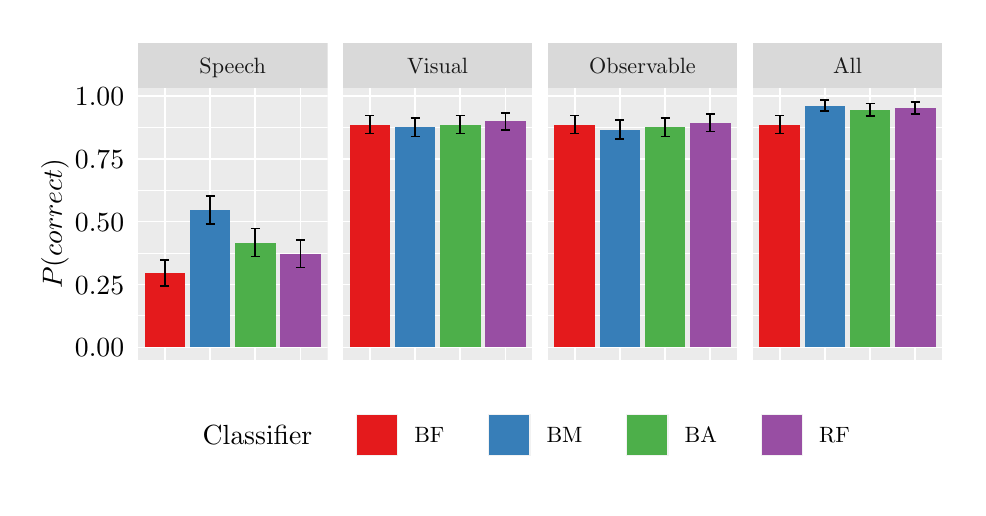
\begin{tikzpicture}[x=1pt,y=1pt]
\definecolor{fillColor}{RGB}{255,255,255}
\path[use as bounding box,fill=fillColor,fill opacity=0.00] (0,0) rectangle (336.00,166.12);
\begin{scope}
\path[clip] (  0.00,  0.00) rectangle (336.00,166.12);
\definecolor{drawColor}{RGB}{255,255,255}
\definecolor{fillColor}{RGB}{255,255,255}

\path[draw=drawColor,line width= 0.6pt,line join=round,line cap=round,fill=fillColor] (  0.00,  0.00) rectangle (336.00,166.12);
\end{scope}
\begin{scope}
\path[clip] ( 39.80, 46.15) rectangle (108.35,144.36);
\definecolor{fillColor}{gray}{0.92}

\path[fill=fillColor] ( 39.80, 46.15) rectangle (108.35,144.36);
\definecolor{drawColor}{RGB}{255,255,255}

\path[draw=drawColor,line width= 0.3pt,line join=round] ( 39.80, 61.97) --
	(108.35, 61.97);

\path[draw=drawColor,line width= 0.3pt,line join=round] ( 39.80, 84.68) --
	(108.35, 84.68);

\path[draw=drawColor,line width= 0.3pt,line join=round] ( 39.80,107.38) --
	(108.35,107.38);

\path[draw=drawColor,line width= 0.3pt,line join=round] ( 39.80,130.09) --
	(108.35,130.09);

\path[draw=drawColor,line width= 0.6pt,line join=round] ( 39.80, 50.61) --
	(108.35, 50.61);

\path[draw=drawColor,line width= 0.6pt,line join=round] ( 39.80, 73.32) --
	(108.35, 73.32);

\path[draw=drawColor,line width= 0.6pt,line join=round] ( 39.80, 96.03) --
	(108.35, 96.03);

\path[draw=drawColor,line width= 0.6pt,line join=round] ( 39.80,118.74) --
	(108.35,118.74);

\path[draw=drawColor,line width= 0.6pt,line join=round] ( 39.80,141.44) --
	(108.35,141.44);

\path[draw=drawColor,line width= 0.6pt,line join=round] ( 49.60, 46.15) --
	( 49.60,144.36);

\path[draw=drawColor,line width= 0.6pt,line join=round] ( 65.92, 46.15) --
	( 65.92,144.36);

\path[draw=drawColor,line width= 0.6pt,line join=round] ( 82.24, 46.15) --
	( 82.24,144.36);

\path[draw=drawColor,line width= 0.6pt,line join=round] ( 98.56, 46.15) --
	( 98.56,144.36);
\definecolor{fillColor}{RGB}{228,26,28}

\path[fill=fillColor] ( 42.25, 50.61) rectangle ( 56.94, 77.50);
\definecolor{fillColor}{RGB}{55,126,184}

\path[fill=fillColor] ( 58.57, 50.61) rectangle ( 73.26,100.30);
\definecolor{fillColor}{RGB}{77,175,74}

\path[fill=fillColor] ( 74.90, 50.61) rectangle ( 89.58, 88.49);
\definecolor{fillColor}{RGB}{152,78,163}

\path[fill=fillColor] ( 91.22, 50.61) rectangle (105.91, 84.31);
\definecolor{drawColor}{RGB}{0,0,0}

\path[draw=drawColor,line width= 0.6pt,line join=round] ( 47.97, 82.22) --
	( 51.23, 82.22);

\path[draw=drawColor,line width= 0.6pt,line join=round] ( 49.60, 82.22) --
	( 49.60, 72.87);

\path[draw=drawColor,line width= 0.6pt,line join=round] ( 47.97, 72.87) --
	( 51.23, 72.87);

\path[draw=drawColor,line width= 0.6pt,line join=round] ( 64.29,105.38) --
	( 67.55,105.38);

\path[draw=drawColor,line width= 0.6pt,line join=round] ( 65.92,105.38) --
	( 65.92, 95.21);

\path[draw=drawColor,line width= 0.6pt,line join=round] ( 64.29, 95.21) --
	( 67.55, 95.21);

\path[draw=drawColor,line width= 0.6pt,line join=round] ( 80.61, 93.49) --
	( 83.87, 93.49);

\path[draw=drawColor,line width= 0.6pt,line join=round] ( 82.24, 93.49) --
	( 82.24, 83.40);

\path[draw=drawColor,line width= 0.6pt,line join=round] ( 80.61, 83.40) --
	( 83.87, 83.40);

\path[draw=drawColor,line width= 0.6pt,line join=round] ( 96.93, 89.31) --
	(100.19, 89.31);

\path[draw=drawColor,line width= 0.6pt,line join=round] ( 98.56, 89.31) --
	( 98.56, 79.41);

\path[draw=drawColor,line width= 0.6pt,line join=round] ( 96.93, 79.41) --
	(100.19, 79.41);
\end{scope}
\begin{scope}
\path[clip] (113.85, 46.15) rectangle (182.40,144.36);
\definecolor{fillColor}{gray}{0.92}

\path[fill=fillColor] (113.85, 46.15) rectangle (182.40,144.36);
\definecolor{drawColor}{RGB}{255,255,255}

\path[draw=drawColor,line width= 0.3pt,line join=round] (113.85, 61.97) --
	(182.40, 61.97);

\path[draw=drawColor,line width= 0.3pt,line join=round] (113.85, 84.68) --
	(182.40, 84.68);

\path[draw=drawColor,line width= 0.3pt,line join=round] (113.85,107.38) --
	(182.40,107.38);

\path[draw=drawColor,line width= 0.3pt,line join=round] (113.85,130.09) --
	(182.40,130.09);

\path[draw=drawColor,line width= 0.6pt,line join=round] (113.85, 50.61) --
	(182.40, 50.61);

\path[draw=drawColor,line width= 0.6pt,line join=round] (113.85, 73.32) --
	(182.40, 73.32);

\path[draw=drawColor,line width= 0.6pt,line join=round] (113.85, 96.03) --
	(182.40, 96.03);

\path[draw=drawColor,line width= 0.6pt,line join=round] (113.85,118.74) --
	(182.40,118.74);

\path[draw=drawColor,line width= 0.6pt,line join=round] (113.85,141.44) --
	(182.40,141.44);

\path[draw=drawColor,line width= 0.6pt,line join=round] (123.65, 46.15) --
	(123.65,144.36);

\path[draw=drawColor,line width= 0.6pt,line join=round] (139.97, 46.15) --
	(139.97,144.36);

\path[draw=drawColor,line width= 0.6pt,line join=round] (156.29, 46.15) --
	(156.29,144.36);

\path[draw=drawColor,line width= 0.6pt,line join=round] (172.61, 46.15) --
	(172.61,144.36);
\definecolor{fillColor}{RGB}{228,26,28}

\path[fill=fillColor] (116.30, 50.61) rectangle (130.99,131.09);
\definecolor{fillColor}{RGB}{55,126,184}

\path[fill=fillColor] (132.62, 50.61) rectangle (147.31,130.18);
\definecolor{fillColor}{RGB}{77,175,74}

\path[fill=fillColor] (148.94, 50.61) rectangle (163.63,131.09);
\definecolor{fillColor}{RGB}{152,78,163}

\path[fill=fillColor] (165.27, 50.61) rectangle (179.95,132.27);
\definecolor{drawColor}{RGB}{0,0,0}

\path[draw=drawColor,line width= 0.6pt,line join=round] (122.01,134.36) --
	(125.28,134.36);

\path[draw=drawColor,line width= 0.6pt,line join=round] (123.65,134.36) --
	(123.65,127.82);

\path[draw=drawColor,line width= 0.6pt,line join=round] (122.01,127.82) --
	(125.28,127.82);

\path[draw=drawColor,line width= 0.6pt,line join=round] (138.34,133.54) --
	(141.60,133.54);

\path[draw=drawColor,line width= 0.6pt,line join=round] (139.97,133.54) --
	(139.97,126.82);

\path[draw=drawColor,line width= 0.6pt,line join=round] (138.34,126.82) --
	(141.60,126.82);

\path[draw=drawColor,line width= 0.6pt,line join=round] (154.66,134.36) --
	(157.92,134.36);

\path[draw=drawColor,line width= 0.6pt,line join=round] (156.29,134.36) --
	(156.29,127.82);

\path[draw=drawColor,line width= 0.6pt,line join=round] (154.66,127.82) --
	(157.92,127.82);

\path[draw=drawColor,line width= 0.6pt,line join=round] (170.98,135.36) --
	(174.24,135.36);

\path[draw=drawColor,line width= 0.6pt,line join=round] (172.61,135.36) --
	(172.61,129.18);

\path[draw=drawColor,line width= 0.6pt,line join=round] (170.98,129.18) --
	(174.24,129.18);
\end{scope}
\begin{scope}
\path[clip] (187.90, 46.15) rectangle (256.45,144.36);
\definecolor{fillColor}{gray}{0.92}

\path[fill=fillColor] (187.90, 46.15) rectangle (256.45,144.36);
\definecolor{drawColor}{RGB}{255,255,255}

\path[draw=drawColor,line width= 0.3pt,line join=round] (187.90, 61.97) --
	(256.45, 61.97);

\path[draw=drawColor,line width= 0.3pt,line join=round] (187.90, 84.68) --
	(256.45, 84.68);

\path[draw=drawColor,line width= 0.3pt,line join=round] (187.90,107.38) --
	(256.45,107.38);

\path[draw=drawColor,line width= 0.3pt,line join=round] (187.90,130.09) --
	(256.45,130.09);

\path[draw=drawColor,line width= 0.6pt,line join=round] (187.90, 50.61) --
	(256.45, 50.61);

\path[draw=drawColor,line width= 0.6pt,line join=round] (187.90, 73.32) --
	(256.45, 73.32);

\path[draw=drawColor,line width= 0.6pt,line join=round] (187.90, 96.03) --
	(256.45, 96.03);

\path[draw=drawColor,line width= 0.6pt,line join=round] (187.90,118.74) --
	(256.45,118.74);

\path[draw=drawColor,line width= 0.6pt,line join=round] (187.90,141.44) --
	(256.45,141.44);

\path[draw=drawColor,line width= 0.6pt,line join=round] (197.69, 46.15) --
	(197.69,144.36);

\path[draw=drawColor,line width= 0.6pt,line join=round] (214.02, 46.15) --
	(214.02,144.36);

\path[draw=drawColor,line width= 0.6pt,line join=round] (230.34, 46.15) --
	(230.34,144.36);

\path[draw=drawColor,line width= 0.6pt,line join=round] (246.66, 46.15) --
	(246.66,144.36);
\definecolor{fillColor}{RGB}{228,26,28}

\path[fill=fillColor] (190.35, 50.61) rectangle (205.04,131.09);
\definecolor{fillColor}{RGB}{55,126,184}

\path[fill=fillColor] (206.67, 50.61) rectangle (221.36,129.27);
\definecolor{fillColor}{RGB}{77,175,74}

\path[fill=fillColor] (222.99, 50.61) rectangle (237.68,130.18);
\definecolor{fillColor}{RGB}{152,78,163}

\path[fill=fillColor] (239.31, 50.61) rectangle (254.00,131.73);
\definecolor{drawColor}{RGB}{0,0,0}

\path[draw=drawColor,line width= 0.6pt,line join=round] (196.06,134.36) --
	(199.33,134.36);

\path[draw=drawColor,line width= 0.6pt,line join=round] (197.69,134.36) --
	(197.69,127.82);

\path[draw=drawColor,line width= 0.6pt,line join=round] (196.06,127.82) --
	(199.33,127.82);

\path[draw=drawColor,line width= 0.6pt,line join=round] (212.38,132.82) --
	(215.65,132.82);

\path[draw=drawColor,line width= 0.6pt,line join=round] (214.02,132.82) --
	(214.02,125.82);

\path[draw=drawColor,line width= 0.6pt,line join=round] (212.38,125.82) --
	(215.65,125.82);

\path[draw=drawColor,line width= 0.6pt,line join=round] (228.71,133.54) --
	(231.97,133.54);

\path[draw=drawColor,line width= 0.6pt,line join=round] (230.34,133.54) --
	(230.34,126.82);

\path[draw=drawColor,line width= 0.6pt,line join=round] (228.71,126.82) --
	(231.97,126.82);

\path[draw=drawColor,line width= 0.6pt,line join=round] (245.03,134.81) --
	(248.29,134.81);

\path[draw=drawColor,line width= 0.6pt,line join=round] (246.66,134.81) --
	(246.66,128.55);

\path[draw=drawColor,line width= 0.6pt,line join=round] (245.03,128.55) --
	(248.29,128.55);
\end{scope}
\begin{scope}
\path[clip] (261.95, 46.15) rectangle (330.50,144.36);
\definecolor{fillColor}{gray}{0.92}

\path[fill=fillColor] (261.95, 46.15) rectangle (330.50,144.36);
\definecolor{drawColor}{RGB}{255,255,255}

\path[draw=drawColor,line width= 0.3pt,line join=round] (261.95, 61.97) --
	(330.50, 61.97);

\path[draw=drawColor,line width= 0.3pt,line join=round] (261.95, 84.68) --
	(330.50, 84.68);

\path[draw=drawColor,line width= 0.3pt,line join=round] (261.95,107.38) --
	(330.50,107.38);

\path[draw=drawColor,line width= 0.3pt,line join=round] (261.95,130.09) --
	(330.50,130.09);

\path[draw=drawColor,line width= 0.6pt,line join=round] (261.95, 50.61) --
	(330.50, 50.61);

\path[draw=drawColor,line width= 0.6pt,line join=round] (261.95, 73.32) --
	(330.50, 73.32);

\path[draw=drawColor,line width= 0.6pt,line join=round] (261.95, 96.03) --
	(330.50, 96.03);

\path[draw=drawColor,line width= 0.6pt,line join=round] (261.95,118.74) --
	(330.50,118.74);

\path[draw=drawColor,line width= 0.6pt,line join=round] (261.95,141.44) --
	(330.50,141.44);

\path[draw=drawColor,line width= 0.6pt,line join=round] (271.74, 46.15) --
	(271.74,144.36);

\path[draw=drawColor,line width= 0.6pt,line join=round] (288.06, 46.15) --
	(288.06,144.36);

\path[draw=drawColor,line width= 0.6pt,line join=round] (304.39, 46.15) --
	(304.39,144.36);

\path[draw=drawColor,line width= 0.6pt,line join=round] (320.71, 46.15) --
	(320.71,144.36);
\definecolor{fillColor}{RGB}{228,26,28}

\path[fill=fillColor] (264.40, 50.61) rectangle (279.09,131.09);
\definecolor{fillColor}{RGB}{55,126,184}

\path[fill=fillColor] (280.72, 50.61) rectangle (295.41,137.90);
\definecolor{fillColor}{RGB}{77,175,74}

\path[fill=fillColor] (297.04, 50.61) rectangle (311.73,136.45);
\definecolor{fillColor}{RGB}{152,78,163}

\path[fill=fillColor] (313.36, 50.61) rectangle (328.05,136.99);
\definecolor{drawColor}{RGB}{0,0,0}

\path[draw=drawColor,line width= 0.6pt,line join=round] (270.11,134.36) --
	(273.38,134.36);

\path[draw=drawColor,line width= 0.6pt,line join=round] (271.74,134.36) --
	(271.74,127.82);

\path[draw=drawColor,line width= 0.6pt,line join=round] (270.11,127.82) --
	(273.38,127.82);

\path[draw=drawColor,line width= 0.6pt,line join=round] (286.43,139.90) --
	(289.70,139.90);

\path[draw=drawColor,line width= 0.6pt,line join=round] (288.06,139.90) --
	(288.06,135.90);

\path[draw=drawColor,line width= 0.6pt,line join=round] (286.43,135.90) --
	(289.70,135.90);

\path[draw=drawColor,line width= 0.6pt,line join=round] (302.75,138.72) --
	(306.02,138.72);

\path[draw=drawColor,line width= 0.6pt,line join=round] (304.39,138.72) --
	(304.39,134.09);

\path[draw=drawColor,line width= 0.6pt,line join=round] (302.75,134.09) --
	(306.02,134.09);

\path[draw=drawColor,line width= 0.6pt,line join=round] (319.08,139.17) --
	(322.34,139.17);

\path[draw=drawColor,line width= 0.6pt,line join=round] (320.71,139.17) --
	(320.71,134.81);

\path[draw=drawColor,line width= 0.6pt,line join=round] (319.08,134.81) --
	(322.34,134.81);
\end{scope}
\begin{scope}
\path[clip] ( 39.80,144.36) rectangle (108.35,160.62);
\definecolor{fillColor}{gray}{0.85}

\path[fill=fillColor] ( 39.80,144.36) rectangle (108.35,160.62);
\definecolor{drawColor}{gray}{0.10}

\node[text=drawColor,anchor=base,inner sep=0pt, outer sep=0pt, scale=  0.80] at ( 74.08,149.74) {Speech};
\end{scope}
\begin{scope}
\path[clip] (113.85,144.36) rectangle (182.40,160.62);
\definecolor{fillColor}{gray}{0.85}

\path[fill=fillColor] (113.85,144.36) rectangle (182.40,160.62);
\definecolor{drawColor}{gray}{0.10}

\node[text=drawColor,anchor=base,inner sep=0pt, outer sep=0pt, scale=  0.80] at (148.13,149.74) {Visual};
\end{scope}
\begin{scope}
\path[clip] (187.90,144.36) rectangle (256.45,160.62);
\definecolor{fillColor}{gray}{0.85}

\path[fill=fillColor] (187.90,144.36) rectangle (256.45,160.62);
\definecolor{drawColor}{gray}{0.10}

\node[text=drawColor,anchor=base,inner sep=0pt, outer sep=0pt, scale=  0.80] at (222.18,149.74) {Observable};
\end{scope}
\begin{scope}
\path[clip] (261.95,144.36) rectangle (330.50,160.62);
\definecolor{fillColor}{gray}{0.85}

\path[fill=fillColor] (261.95,144.36) rectangle (330.50,160.62);
\definecolor{drawColor}{gray}{0.10}

\node[text=drawColor,anchor=base,inner sep=0pt, outer sep=0pt, scale=  0.80] at (296.23,149.74) {All};
\end{scope}
\begin{scope}
\path[clip] (  0.00,  0.00) rectangle (336.00,166.12);
\definecolor{drawColor}{RGB}{0,0,0}

\node[text=drawColor,anchor=base east,inner sep=0pt, outer sep=0pt, scale=  1.00] at ( 34.85, 47.17) {0.00};

\node[text=drawColor,anchor=base east,inner sep=0pt, outer sep=0pt, scale=  1.00] at ( 34.85, 69.88) {0.25};

\node[text=drawColor,anchor=base east,inner sep=0pt, outer sep=0pt, scale=  1.00] at ( 34.85, 92.59) {0.50};

\node[text=drawColor,anchor=base east,inner sep=0pt, outer sep=0pt, scale=  1.00] at ( 34.85,115.29) {0.75};

\node[text=drawColor,anchor=base east,inner sep=0pt, outer sep=0pt, scale=  1.00] at ( 34.85,138.00) {1.00};
\end{scope}
\begin{scope}
\path[clip] (  0.00,  0.00) rectangle (336.00,166.12);
\definecolor{drawColor}{RGB}{0,0,0}

\node[text=drawColor,rotate= 90.00,anchor=base,inner sep=0pt, outer sep=0pt, scale=  1.00] at ( 12.39, 95.26) {\(P(correct)\)};
\end{scope}
\begin{scope}
\path[clip] (  0.00,  0.00) rectangle (336.00,166.12);
\definecolor{fillColor}{RGB}{255,255,255}

\path[fill=fillColor] ( 57.74,  5.50) rectangle (312.57, 32.40);
\end{scope}
\begin{scope}
\path[clip] (  0.00,  0.00) rectangle (336.00,166.12);
\definecolor{drawColor}{RGB}{0,0,0}

\node[text=drawColor,anchor=base west,inner sep=0pt, outer sep=0pt, scale=  1.00] at ( 63.24, 15.51) {Classifier};
\end{scope}
\begin{scope}
\path[clip] (  0.00,  0.00) rectangle (336.00,166.12);
\definecolor{drawColor}{RGB}{255,255,255}
\definecolor{fillColor}{gray}{0.95}

\path[draw=drawColor,line width= 0.6pt,line join=round,line cap=round,fill=fillColor] (118.31, 11.00) rectangle (134.21, 26.90);
\end{scope}
\begin{scope}
\path[clip] (  0.00,  0.00) rectangle (336.00,166.12);
\definecolor{fillColor}{RGB}{228,26,28}

\path[fill=fillColor] (119.02, 11.71) rectangle (133.50, 26.19);
\end{scope}
\begin{scope}
\path[clip] (  0.00,  0.00) rectangle (336.00,166.12);
\definecolor{drawColor}{RGB}{255,255,255}
\definecolor{fillColor}{gray}{0.95}

\path[draw=drawColor,line width= 0.6pt,line join=round,line cap=round,fill=fillColor] (166.10, 11.00) rectangle (182.00, 26.90);
\end{scope}
\begin{scope}
\path[clip] (  0.00,  0.00) rectangle (336.00,166.12);
\definecolor{fillColor}{RGB}{55,126,184}

\path[fill=fillColor] (166.81, 11.71) rectangle (181.29, 26.19);
\end{scope}
\begin{scope}
\path[clip] (  0.00,  0.00) rectangle (336.00,166.12);
\definecolor{drawColor}{RGB}{255,255,255}
\definecolor{fillColor}{gray}{0.95}

\path[draw=drawColor,line width= 0.6pt,line join=round,line cap=round,fill=fillColor] (215.99, 11.00) rectangle (231.89, 26.90);
\end{scope}
\begin{scope}
\path[clip] (  0.00,  0.00) rectangle (336.00,166.12);
\definecolor{fillColor}{RGB}{77,175,74}

\path[fill=fillColor] (216.71, 11.71) rectangle (231.18, 26.19);
\end{scope}
\begin{scope}
\path[clip] (  0.00,  0.00) rectangle (336.00,166.12);
\definecolor{drawColor}{RGB}{255,255,255}
\definecolor{fillColor}{gray}{0.95}

\path[draw=drawColor,line width= 0.6pt,line join=round,line cap=round,fill=fillColor] (264.56, 11.00) rectangle (280.46, 26.90);
\end{scope}
\begin{scope}
\path[clip] (  0.00,  0.00) rectangle (336.00,166.12);
\definecolor{fillColor}{RGB}{152,78,163}

\path[fill=fillColor] (265.27, 11.71) rectangle (279.75, 26.19);
\end{scope}
\begin{scope}
\path[clip] (  0.00,  0.00) rectangle (336.00,166.12);
\definecolor{drawColor}{RGB}{0,0,0}

\node[text=drawColor,anchor=base west,inner sep=0pt, outer sep=0pt, scale=  0.80] at (139.71, 16.19) {BF  };
\end{scope}
\begin{scope}
\path[clip] (  0.00,  0.00) rectangle (336.00,166.12);
\definecolor{drawColor}{RGB}{0,0,0}

\node[text=drawColor,anchor=base west,inner sep=0pt, outer sep=0pt, scale=  0.80] at (187.50, 16.19) {BM  };
\end{scope}
\begin{scope}
\path[clip] (  0.00,  0.00) rectangle (336.00,166.12);
\definecolor{drawColor}{RGB}{0,0,0}

\node[text=drawColor,anchor=base west,inner sep=0pt, outer sep=0pt, scale=  0.80] at (237.39, 16.19) {BA  };
\end{scope}
\begin{scope}
\path[clip] (  0.00,  0.00) rectangle (336.00,166.12);
\definecolor{drawColor}{RGB}{0,0,0}

\node[text=drawColor,anchor=base west,inner sep=0pt, outer sep=0pt, scale=  0.80] at (285.96, 16.19) {RF  };
\end{scope}
\end{tikzpicture}
